%!TEX root = ../paper.tex

\section{Implementation}
\label{sec:implementation}

This section will present our implementations for the demand and product classifier.
We will start with describing our example data set.

\subsection{Example Data Set}
\label{sub:initial_data_set}
We implemented a prototype of our \nto system based on data from a Germany software company called SAP.
SAP is the biggest software vendor in Europe and builds software for both small and large enterprises.
SAP provided us with nearly 100 brochures about four SAP software products, which are explained in Table~\ref{table:products}.
We chose LinkedIn as the business-oriented social network, as it is the biggest and most popular platform.
We crawled approximately 19,000 posts from LinkedIn.

Unfortunately, around 75~\% of the brochures are in German and the LinkedIn posts are written in English.
To solve the language mismatch, we translated the documents with an machine translation tools and replaced the German brochures with its translations.
Additionally, we added some book descriptions from Amazon about these products to enlarge the training set.

\begin{table}[h]
	\centering
	{
		\renewcommand\arraystretch{1.25}
		\begin{tabular}{lll}
			\hline
			\textbf{Product} & \multicolumn{2}{l}{\textbf{Explanation}} \\
			\hline\hline
			CRM  & \multicolumn{2}{p{10cm}}{\raggedright
				Customer relationship management software helps to manage a company's interactions with past, present, and future potential customers.} \\
			\hline
			ECOM  & \multicolumn{2}{p{10cm}}{\raggedright
				Ecommerce software helps to automatize sale processes in the context of internet companies.} \\
			\hline
			HCM  & \multicolumn{2}{p{10cm}}{\raggedright
				Human capital management software supports the company in managing human resources and helps in recruitment and employee management.} \\
			\hline
			LVM  & \multicolumn{2}{p{10cm}}{\raggedright
				Landscape virtualization management software helps to deploy and manage existing applications in virtualized data centers and cloud infrastructures.} \\
			\hline
		\end{tabular}
	}
	\caption{Different products in the training data set of SAP brochures.}
	\label{table:products}
\end{table}

\subsection{Manual Annotation of LinkedIn Posts}

At the moment, there exists no data set for a demand classification, which can be used for learning and evaluation purposes.
Therefore, we tagged some post manually.
We used an active learning approach to create the gold standard for both training and evaluation.
In an active learning setting, the algorithm ``asks an oracle, typically a human with extensive knowledge of the domain at hand, about [...] the instances for which the model [...] makes unreliable predictions'' \cite{olsson2009literature}.
First, we randomly tagged some posts, then we built a basic classifier, which we ran over all posts to finally ask for a tagging decision for the most unsure post.
Then we reran the classification and the classifier asked again.
Using this approach, we are able to get the most out of our limited tagging time.
The results of the tagging can be found in Table~\ref{table:data_overview}.

\begin{table}[h]
	\centering
	\begin{tabular}{lcc}
		\hline
		\textbf{Class} & \textbf{Number of posts} & \textbf{Percentage} \\
		\hline
		\hline
		$\operatorname{demand}$ & 39 & 8.76~\% \\
		\hline
		$\operatorname{no-demand}$ & 406 & 91.24~\% \\
		\hline
		\hline
		$\operatorname{CRM}$ & 18 & 4.05~\% \\
		\hline
		$\operatorname{ECOM}$ & 6 & 1.35~\% \\
		\hline
		$\operatorname{HCM}$ & 19 & 4.27~\% \\
		\hline
		$\operatorname{LVM}$ & 54 & 12.14~\% \\
		\hline
		$\operatorname{no-product}$ & 348 & 78.20~\% \\
		\hline
	\end{tabular}
	\caption{Number of posts in each tagging class.}
	\label{table:data_overview}
\end{table}

We built a tagging web app which implements the active learning.
All together, we tagged about 350 LinkedIn posts, both in respect of demand and product.
In an initial step, each post was tagged by at least two different persons to avoid misclassifications because of the opinion of one tagger.
If there were conflicts between the tagging decisions, a third person was tagging again to solve the conflict.
To evaluate the demand classifier, we use a ten-fold cross validation of all posts, because we need the posts also for training.
To evaluate the product classifier, we can use all annotated posts, because we are learning on the brochures.

\subsection{Demand Classifier}
For the demand classifier, we added the following manually built features, which have been shown to increase the overall performance:
\begin{itemize}
	\item Number of questions in the post. Demand posts usually have more questions.
	\item Number of imperatives in the post. Demand posts usually have more imperatives like ``Please help me out'' or ``Give me advice''.
	\item Whether an e-mail address was given in the post. Demand posts often give an e-mail address to send answers to.
\end{itemize}

\todo{Why Na\"{i}ve Bayes classifier? Evaluate other classifier! Copy stuff from slides.}
We decided on a Na\"{i}ve Bayes classifier with a Bernoulli event model.
The bernoulli event model is especially suited for the demand classification task.
As all Na\"{i}ve Bayes approaches it assumes, that all features are independent of each other.
Equation~\ref{equation:bernoulli} shows the formula for the conditional probability in the Bernoulli Na\"{i}ve Bayes.
The probability that a document $d$ belongs to a class $C$ is calculated with respect to the entire vocabulary set.
This especially means, that a term influences the probability, even if it is not in the document.
This works good with our feature selection, as we also select feature terms based on their non-occurrence.

\captionsetup{singlelinecheck=off}
\begin{equationBlock}
\begin{align*}
	p(d|C) &= \prod_{w~\epsilon~V} bernoulli(w, d, C) \\
	bernoulli(w, d, C) &=
	\begin{cases}
		p(w|C) 					&\text{if w in d}\\
		\overline{p(w|C)} 		&\text{otherwise}
	\end{cases}
	\end{align*}
	\caption{
		Bernoulli Na\"{i}ve Bayes~\cite{mccallum1998comparison} definition.
		It describes the probability that a document $d$ is generated for class $C$.
		A document consists of terms $w$.
		The set of all terms $w$ forms the vocabulary $V$.
	}
	\label{equation:bernoulli}
\end{equationBlock}

\subsection{Product Classifier}
For the product classifier we evaluated several classifiers and variants of the feature vector using the most important words as features as described in Section~\ref{sub:feature-selection}.
The results are shown in Figure~\ref{fig:product-classifier}.
In general, the linear classifiers like Logistic Regression, SVM, and Perceptron perform better than the others.
Therefore, we decide to use a linear classifier.

We tested two additional parameters for the classifcation process:
\begin{itemize}
	\item
		\textbf{Binarization}:
			When using binarization, we count each feature only once per document, e.g. if a word occurs several times, we still count it as if it occured only once.
	\item
		\textbf{Normalization}:
			When using normalization, we normalize the resulting feature vector to a sum of one.
\end{itemize}
As Figure~\ref{fig:product-classifier} shows, using binarization and normalization in general improves the result for the linear classifiers.

\begin{figure}
	\centering
	\begin{subfigure}[t]{0.3\textwidth}
		\centering
		\begin{tabular}{r | r | r}
			& \textbf{N} 	& \textbf{\textoverline{N}}\\
			\hline
			\textbf{B} 					& 74.1~\%		& 72.5~\% \\
			\textbf{\textoverline{B}}	& 73.3~\% 		& 72.5~\% \\
		\end{tabular}
		\caption{Logistic Regression~\cite{leCessie1992}}
	\end{subfigure}~
	\begin{subfigure}[t]{0.3\textwidth}
		\centering
		\begin{tabular}{r | r | r}
			& \textbf{N} 	& \textbf{\textoverline{N}}\\
			\hline
			\textbf{B} 					& 80.0~\%		& 75.0~\% \\
			\textbf{\textoverline{B}}	& 75.8~\% 		& 62.5~\% \\
		\end{tabular}
		\caption{Support Vector Machine~\cite{Platt1998}}
	\end{subfigure}~
	\begin{subfigure}[t]{0.3\textwidth}
		\centering
		\begin{tabular}{r | r | r}
			& \textbf{N} 	& \textbf{\textoverline{N}}\\
			\hline
			\textbf{B} 					& 70.8~\%		& 70.0~\% \\
			\textbf{\textoverline{B}}	& 60.8~\% 		& 60.8~\% \\
		\end{tabular}
		\caption{Multilayer Perceptron~\cite{ruck1990multilayer}}
		\center
	\end{subfigure}

	\begin{subfigure}[t]{0.3\textwidth}
		\centering
		\begin{tabular}{r | r | r}
			& \textbf{N} 	& \textbf{\textoverline{N}}\\
			\hline
			\textbf{B} 					& 68.3~\%		& 70.0~\% \\
			\textbf{\textoverline{B}}	& 70.0~\% 		& 75.8~\% \\
		\end{tabular}
		\caption{J48 Decision Tree~\cite{Quinlan1993}}
	\end{subfigure}~
	\begin{subfigure}[t]{0.3\textwidth}
		\centering
		\begin{tabular}{r | r | r}
			& \textbf{N} 	& \textbf{\textoverline{N}}\\
			\hline
			\textbf{B} 					& 67.5~\%		& 56.7~\% \\
			\textbf{\textoverline{B}}	& 68.3~\% 		& 48.3~\% \\
		\end{tabular}
		\caption{Nearest Neighbour~\cite{Aha1991}}
	\end{subfigure}~
	\begin{subfigure}[t]{0.3\textwidth}
		\centering
		\begin{tabular}{r | r | r}
			& \textbf{N} 	& \textbf{\textoverline{N}}\\
			\hline
			\textbf{B} 					& 48.3~\%		& 56.7~\% \\
			\textbf{\textoverline{B}}	& 57.5~\% 		& 27.5~\% \\
		\end{tabular}
		\caption{Bernoulli Naive Bayes~\cite{John1995}}
	\end{subfigure}~
	\caption{Precision of the classifier. N indicates whether the feature vector was normalized with the L1-Norm. B indicates whether we use binary features per document. The linear classifiers like logistic regression, svm, and perceptron perform best.}
	\label{fig:product-classifier}
\end{figure}

\subsection{Sampling Algorithm}
As already mentioned in the previous sections, we extend our training set further by splitting the brochures and Amazon product texts into smaller chunks.
We did this to solve the \emph{document mismatch} and \emph{small corpus problem}.
In the following, we compare two different splitting strategies:
\begin{itemize}
	\item
		\textbf{Grouping:}
		We split each brochure into groups of $k$ sentences.
		It is important to note, that groups are disjoint, i.e. no sentence appears in two different groups.
		If there are less than $k$ sentences left at the end, we simply build a brochure of the remaining sentences.
		For example, if one brochure contains 15 sentences and we split into groups of six, we end up with three brochures with six, six, and three sentences respectively.
	\item
		\textbf{Sliding:}
		We move a sliding window of size $k$ over the sentences in one group.
		Thereby, one sentence occurs in several windows and hence in several brochures at the end.
		If we have eight sentences, and a window size of six, we end up with three documents $1 - 6$, $2 - 7$, and $3 - 8$.
		Obviously, there are more brochures here, but also more duplicate sentences.
\end{itemize}

We evaluated these two strategies for different values of $k$, see Figure~\ref{fig:sampling_optimization}.
We received the best results for grouping and $k = 6$.
Of course this value largely depends on the concrete data set at hand, so this optimization needs to be done again for every application of our \nto approach.

\begin{figure}
	\begin{center}
		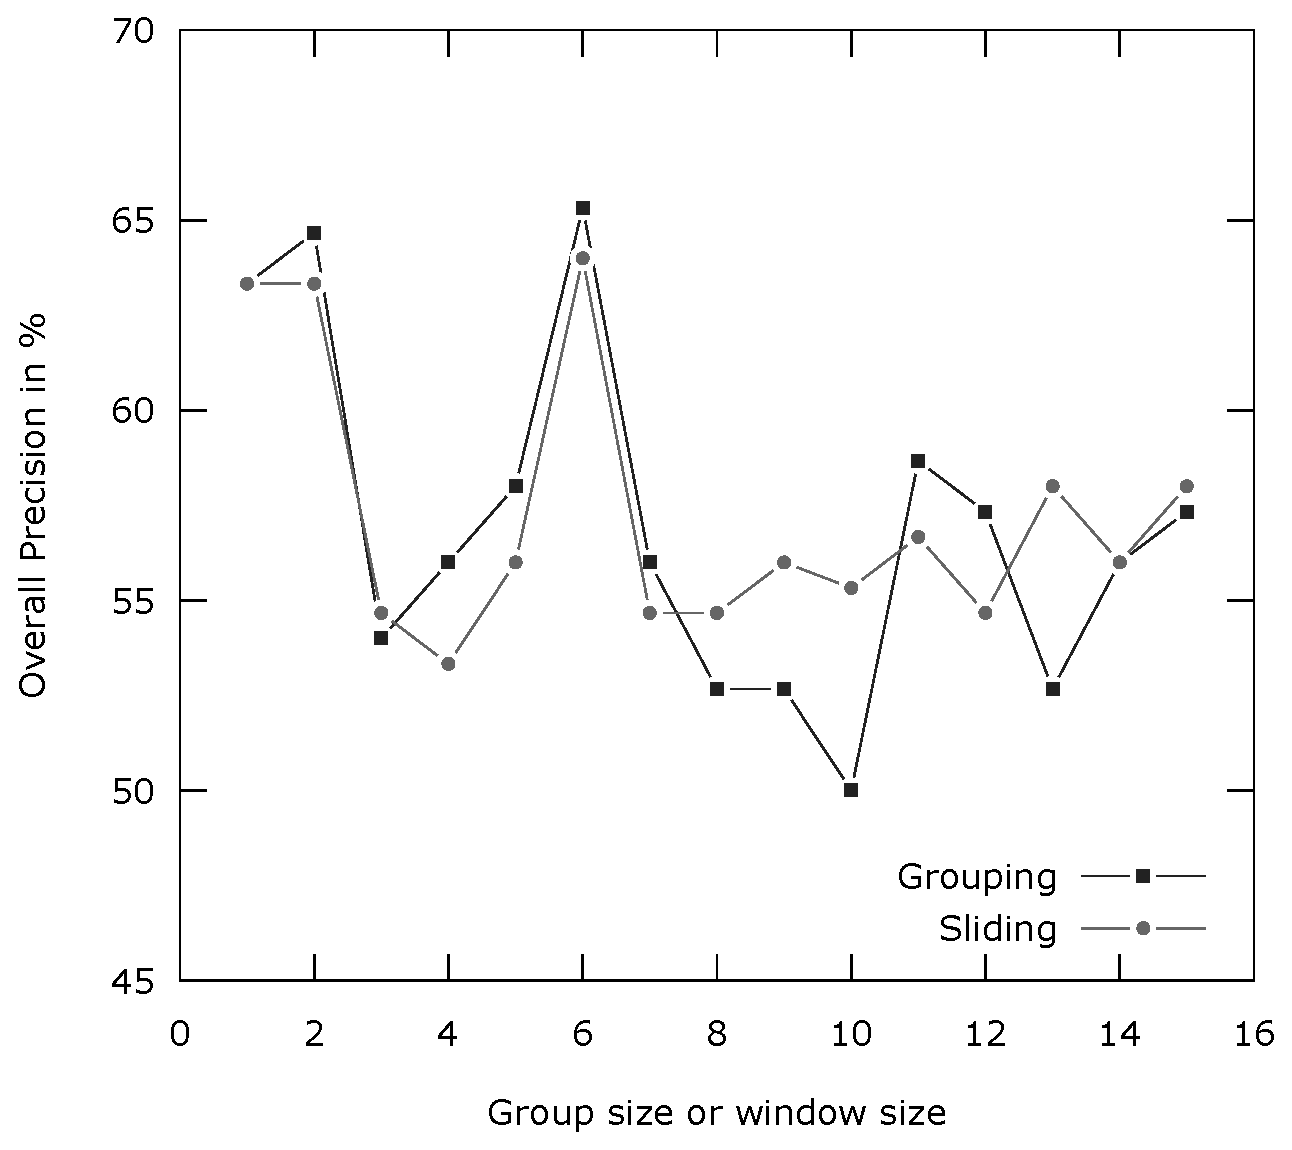
\includegraphics[width=0.6\textwidth]{figures/sampling_optimization.eps}
	\end{center}
	\caption{Comparing grouping and sliding for different group sizes/window sizes. Plotted against the overall precision of the system, i.e. how many of the predictions were correct. The best results were obtained for $k$ and the grouping strategy.}
	\label{fig:sampling_optimization}
\end{figure}
